\chapter{Observed catalogue and held-out diagnostics}
\label{ch:observed}

\section{Scope and provenance of the archived catalogue}

The empirical analysis begins with an archived catalogue rather than with the unavailable inputs to the original manuscript. The primary archive is a GeoNet WFS snapshot downloaded on 15 October 2026. Events were selected with magnitude \(M\geq 5\) and depth no greater than \(40\)~km, within latitude \([-48.5,-33.5]\) and longitude \([165,180]\). The depth sentinel value \(-9\) was excluded, while other negative depths were retained. The resulting file contains 913 selected events in a 24,394-day observation window, from 1960-01-01 inclusive to 2026-10-15 exclusive. The event count is recorded, together with the filter definition and catalogue metadata, in the archived research report and processed metadata (\hyperlink{S25}{archival \texttt{S25} (not distributed)}; \href{https://github.com/Drefetr/InhibitoryEarthquakeModels/blob/3e76a174cf4f58ce601c6c9640c4d0c11168813f/provenance/catalogue_snapshot_metadata.json}{public metadata extract} (\texttt{S24})).

The reappearance of the number 913 does not establish identity with the event list analysed in the original work. The original frozen data, source configuration, and executable code are absent, so neither event identity nor processing history can be recovered. A second archived FDSN interface from the same provider returned 914 selections, consisting of 913 events common to the primary snapshot and the additional event 2025p672513. These are interface selections from one national provider, not independent physical catalogues. The interfaces share the same provider and much of their processing history; agreement between them cannot serve as independent validation of completeness or magnitude accuracy.

This distinction governs the interpretation of every later comparison. The reconstruction is an independent analysis applied to a documented archive snapshot, not a numerical replay of the historical analysis. The fitted catalogue slope for a continuous excess-exponential magnitude model is \(2.849401764894274\). For comparison with the earlier manuscript's half-bin convention, define
\[
 \widehat\beta_{\mathrm{adj}}
 =\frac{1}{\overline{M-M_0}+0.05},\qquad M_0=5.
\]
Applied to the archived selection, this gives \(2.494071218330174\), consistent in rounded form with the reported value near \(2.494\). This reconciles an estimator convention; mixed precision and native magnitude scales do not establish a common half-bin adjustment as a generally validated correction for this catalogue. The primary continuous estimate, raw magnitudes, productivity normalization and fitted-law records remain unchanged. It does not demonstrate that the historical event sample or likelihood calculation has been reproduced. Completeness above a time-varying threshold, the relation between native magnitude scales, missing parents of smaller or deeper events, activity before 1960, and the adequacy of national pooling therefore remain explicit assumptions (\hyperlink{S27}{archival \texttt{S27} (not distributed)}).


\begin{figure}[tbp]
\centering
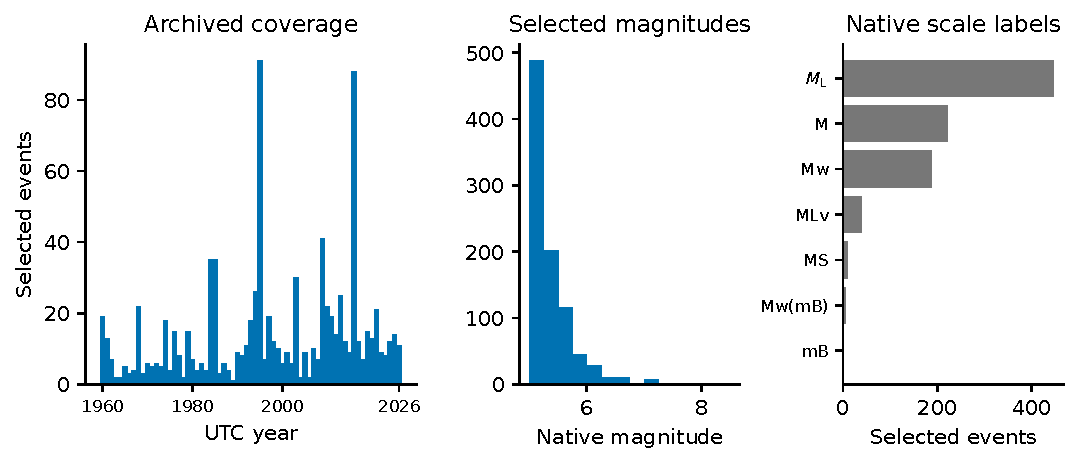
\includegraphics[width=\linewidth]{catalogue.pdf}
\caption{Descriptive summaries of the 913-event archived selection: annual counts, magnitudes and native magnitude labels. The final calendar year is partial. These plots describe this selection and do not establish catalogue completeness or homogeneous observation through time.}
\label{fig:catalogue}
\end{figure}

\section{A restricted diagnostic intensity}

The observed comparison uses the temporal diagnostic defined in the experimental design:
\begin{equation}
 \lambda_\eta(t)=B(t)e^{-\eta G_s(t)}+nH_e(t),\qquad
 B(t)=e^{a+d(2t/T_0-1)},\quad \eta\geq0.
 \label{eq:observed-diagnostic}
\end{equation}
Here the subscript \(s\) denotes stress memory and \(e\) denotes excitation. Neither denotes a spatial coordinate. Both features depend only on strictly earlier events. The implemented Mittag--Leffler (ML) kernels are finite positive spectral mixtures. A shared-memory recipe supplies the same kernel parameters to the stress and triggering features, although those features enter different parts of the intensity. The background is specified independently of the stress history. Thus this family diagnoses a restricted form of inhibition; it does not reproduce the original physical loading construction.

The five observed candidate families were constant Poisson, loglinear Poisson, Omori triggering, ML triggering, and ML triggering with shared inhibition. The principal contrasts compare the last three families. Model labels use ``ML'' for Mittag--Leffler. The native local-magnitude label in Figure~\ref{fig:catalogue} is displayed as \(M_{\mathrm L}\); the original archive label is retained in the data. All five families and their search rules are recorded in \href{https://github.com/Drefetr/InhibitoryEarthquakeModels/blob/3e76a174cf4f58ce601c6c9640c4d0c11168813f/engine/iteration_27/configs/observed_frozen.json}{public search protocol (operational adaptation)} (\texttt{S18}).

The temporal Omori comparator uses the normalized triggering density
\[
 h_{\mathrm O}(u;c,p)=\frac{p-1}{c}\left(1+\frac{u}{c}\right)^{-p}
 =(p-1)c^{p-1}(u+c)^{-p},
 \qquad u\geq0,\quad c>0,\quad p>1.
\]
The lag \(u\) is measured in days. Its integral on $[0,\infty)$ is one. The scale $c$ is measured in days and
is stored as \texttt{KernelSpec.tau}; the triggering multiplier $n$ remains
separate. This specifies the temporal comparator used here, not a complete
space--time ETAS construction.

The split is chronological. The absolute trend coordinate is \(x=2t/T_0-1\), where \(T_0=24394\) days. Candidate fits use the first \(0.50\), \(0.65\), and \(0.80\) fractions of the archive horizon as training prefixes, comprising 301, 504, and 659 events. Tests use the following disjoint intervals \(0.50\)--\(0.65\), \(0.65\)--\(0.80\), and \(0.80\)--\(1.00\), containing 203, 155, and 254 events and 612 test events in total. These intervals correspond approximately to 1993--2003, 2003--2013, and 2013--2026, but the fractions and archive day indices are the operative definitions.

All retained history before each origin, including earlier test history, is available to the candidate intensity. Each fit uses only its training prefix. The exponential mark-rate estimate is obtained from training marks alone and is common across candidate families; it is a plug-in estimate rather than a joint marked-intensity maximum-likelihood estimate. The reported score is the full marked-event score: the sum of event log intensities and log mark densities minus the integrated intensity over quiet exposure, with the final censor handled explicitly in the declared protocol. The uninhibited fit is retained as an exact eligible point in the inhibited search, so nonnegative training gain is partly built into candidate selection. This fact limits any inference from training improvement alone. The stored training gains for the shared diagnostic are \(2.731009\), \(0.302486\), and \(0.143866\), but those numbers are not treated as evidence of predictive success.

\subsection{Saved parameters at the predictive origins}\label{sec:saved-fits}
Table~\ref{tab:saved-predictive-parameters} displays the saved selected records for the three triggering families at the three predictive origins, not new fits. The \href{https://github.com/Drefetr/InhibitoryEarthquakeModels/blob/3e76a174cf4f58ce601c6c9640c4d0c11168813f/paper/supplements/predictive_parameters.json}{selected-parameter companion}
% Exact companion path: supplements/predictive_parameters.json
 retains all fifteen records for the five families, full precision, source hashes and field pointers. The constant Poisson model fixes \(d=n=\eta=0\); loglinear Poisson fixes \(n=\eta=0\). The table's two uninhibited triggering families fix \(\eta=0\).

\begin{table}[htbp]
\centering\small
\setlength{\tabcolsep}{4pt}
\caption{Saved selected parameters at three predictive origins. The background is \(\exp(a+dz(t)-\eta G_s(t))\) per day, with \(z(t)=2t/24394-1\). Values are rounded for display; zeros in the uninhibited families are fixed.}
\label{tab:saved-predictive-parameters}
\begin{tabular}{llrrrr}
\toprule Origin & Family & \(a\) & \(d\) & \(n\) & \(\eta\) \\ \midrule
50\% & Omori & $-4.712517$ & $-0.457071$ & 0.685640 & 0.000000 \\
50\% & Mittag--Leffler & $-4.458572$ & $-0.252150$ & 0.455824 & 0.000000 \\
50\% & Shared inhibition & $-2.196743$ & 1.789757 & 0.481700 & 1.646714 \\
65\% & Omori & $-4.291554$ & 0.048036 & 0.570076 & 0.000000 \\
65\% & Mittag--Leffler & $-4.188810$ & 0.147441 & 0.497996 & 0.000000 \\
65\% & Shared inhibition & $-3.841844$ & 0.492682 & 0.503490 & 0.211710 \\
80\% & Omori & $-4.394252$ & $-0.196162$ & 0.561216 & 0.000000 \\
80\% & Mittag--Leffler & $-4.282575$ & $-0.056651$ & 0.470292 & 0.000000 \\
80\% & Shared inhibition & $-4.103408$ & 0.127638 & 0.473071 & 0.105254 \\
\bottomrule
\end{tabular}
\par\medskip
\begin{tabular}{lrrrr}
\toprule Origin & \(\beta_{\rm train}\) & \(r\) & Omori \(c\) (days) & Omori \(p\) \\ \midrule
50\% & 3.101622 & 0.4 & 0.012995 & 1.113368 \\
65\% & 3.149488 & 0.7 & 0.020798 & 1.198604 \\
80\% & 3.021907 & 0.7 & 0.006972 & 1.155845 \\
\bottomrule
\end{tabular}
\end{table}

All six selected Mittag--Leffler kernels use \(\alpha=0.5\), the lower searched grid endpoint, and \(\tau=1\) day, an interior grid value. The common selected productivity ratio is \(r=0.4\) at the first origin and \(r=0.7\) at the later origins; the former is the lower searched ratio endpoint. The Omori coordinates \(c,p\) were optimized continuously with a retained coarse-grid floor; they are not merely grid winners. These endpoint descriptions are newly checked arithmetic against the frozen search grids. Historical boundary flags, tolerance-based near-boundary classifications and standard errors were not saved. The selected continuous coordinates are strictly inside their recorded bounds under exact comparison. No uncertainty estimates are inferred.

The rates \(\beta_{\rm train}\) are estimated from training marks alone, held common across families, and frozen during each test. Inactive serialization fields are not fitted coordinates: the saved \(p\) field of a Mittag--Leffler kernel and \(\alpha\) field of an Omori kernel have no role in their respective formulas. 

At the three predictive origins, the selected shared-inhibition recipe's
unattenuated deterministic background is approximately \(9.60\), \(1.57\)
and \(1.34\) times that of the corresponding noninhibited Mittag--Leffler
recipe, respectively. The first-origin fit therefore combines a much larger
baseline with stronger depletion. These are descriptive ratios of fitted
components, not total-intensity ratios or a demonstrated causal explanation
of the subsequent predictive loss.

\section{Earlier calibrated restrictions}

The earlier reconstructed analysis tested two restrictions: no feedback and a common rather than separate memory scale. Its observed statistics were \(0.7036472\) and \(0.0829952\), respectively. The completed fitted-law calibration retained \(1{,}999\) null cases per restriction, giving add-one ranks of \(0.365\) and \(0.263\). Neither restriction was rejected by that declared five-percent procedure. These are conditional ranks, not probabilities that the hypotheses are true. In particular, non-rejection does not demonstrate equal physical memories, and the stress kernel's disappearance at zero feedback limits what such a restriction can establish. The calibration authority is \hyperlink{S01}{archival \texttt{S01} (not distributed)}; its interpretation is summarized in \hyperlink{S27}{archival \texttt{S27} (not distributed)}.

The later chronological comparison asks a different question: do the declared inhibited recipes predict subsequent observations better than serious triggering alternatives? A negative predictive result need not contradict a non-rejecting in-sample restriction test. Their targets, fitting rules and calibration differ.

\section{Held-out score comparison}

Table~\ref{tab:observed-scores} reports score differences relative to the ML triggering-only benchmark. Negative values favour the benchmark; positive values favour the named alternative.

\begin{table}[!ht]
\centering
\caption{Held-out marked-process score differences relative to the ML triggering-only benchmark. Tests are disjoint chronological intervals in the declared archive protocol. Values are differences, not log-likelihoods for separate datasets.}
\label{tab:observed-scores}
\small
\setlength{\tabcolsep}{4pt}
\begin{tabular}{lrrrr}
\toprule
Contrast & Test 1 & Test 2 & Test 3 & Total \\
\midrule
Shared inhibition \(-\) ML & \(-16.517557\) & \(-0.075277\) & \(-1.030025\) & \(-17.622859\) \\
Omori triggering-only \(-\) ML & \(+3.106623\) & \(+2.837708\) & \(+6.513790\) & \(+12.458121\) \\
\bottomrule
\end{tabular}
\end{table}

The shared diagnostic loses in all three folds. Its total disadvantage is driven overwhelmingly by the first block: approximately \(93.7\%\) of the total deficit occurs there. The second-block difference is nearly zero, but that is not strong independent evidence of parity because the training histories overlap and later folding choices were inspected during development. The calculations are exploratory and were not designed as confirmatory or as an independent sequence of repeated tests (\hyperlink{S19}{archival \texttt{S19} (not distributed)}).

The continuous Omori recipe improves on the finite ML kernel grid in every fold. This result cannot be converted into a universal law ranking. The Omori refinement and the finite spectral ML candidate have unequal flexibility, and the contrast therefore favours the declared Omori recipe under its fitting convention. It is not an isolated estimate of the effect of \(\eta\), nor a demonstration that every continuously refined triggering model dominates every grid-based alternative. Residual diagnostics were descriptive, varied over the record, and did not certify any winner as an adequate physical model.


\begin{figure}[tbp]
\centering
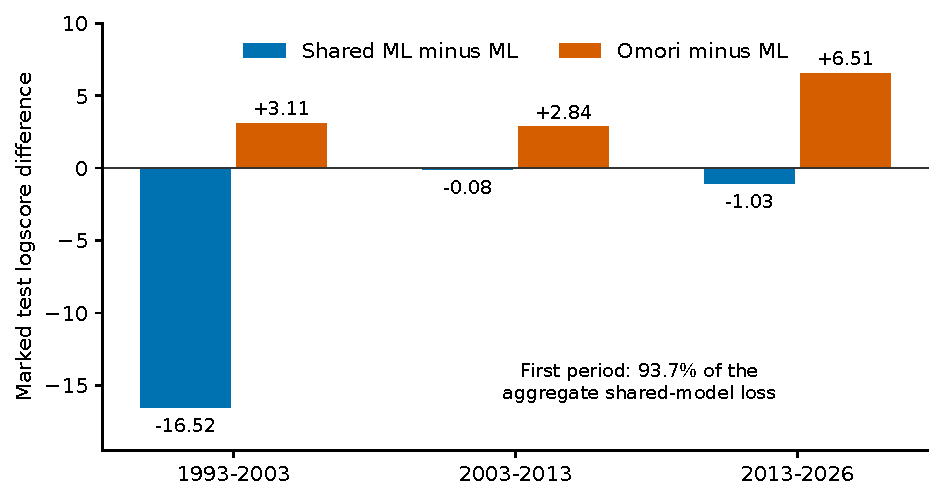
\includegraphics[width=\linewidth]{prediction.pdf}
\caption{Chronological test-score contrasts for the declared recipes. The first test block contributes about 93.7\% of the aggregate shared-inhibition disadvantage. Training prefixes overlap and the periods were reused in exploratory development; the three periods are not independent confirmatory tests.}
\label{fig:prediction}
\end{figure}

\section{Score accounting and temporal localization}

For a fold, write the score difference as
\begin{equation}
  \Delta\ell
  = E+C,
  \qquad
  E=\sum_i\log\frac{\lambda_{\mathrm{sh},i}}{\lambda_{\mathrm{ML},i}},
  \qquad
  C=\Lambda_{\mathrm{ML}}-\Lambda_{\mathrm{sh}},
  \label{eq:score-accounting}
\end{equation}
where the event sum uses pre-event intensities at the realized times, and \(\Lambda\) denotes the corresponding integrated intensity. This separates event-term disagreement from realized compensator disagreement. In the first test block,
\[
E=-33.715205,\qquad C=17.197647,\qquad \Delta\ell=-16.517557.
\]
The integrated intensities are \(115.871595\) under the shared diagnostic and \(133.069242\) under the ML benchmark for 203 events. These are not conventional expected counts from a fixed fitted Poisson model: the compensator is evaluated along an updating estimated history. Its realized value is not automatically the future expected count conditional only on information at the test origin. No naive Poisson count probability value is attached to their difference.

Four equal-duration bins within the first test interval sharpen the accounting without allocating events to bins by any counterfactual rule. Each bin uses the complete preceding history and integrates over its own realized path. Approximate calendar labels are displayed only for orientation; the archive-day boundaries define the calculation.

\begin{table}[!ht]
\centering
\caption{Score accounting within four equal-duration subintervals of the first test block. Each row uses full preceding history and realized integration within that subinterval.}
\label{tab:first-block-accounting}
\small
\setlength{\tabcolsep}{4pt}
\begin{tabular}{lrrr}
\toprule
Approximate interval & \(E\) & \(C\) & \(\Delta\ell\) \\
\midrule
1993-05-24 to 1995-11-24 & \(-2.891244\) & \(2.464270\) & \(-0.426975\) \\
1995-11-24 to 1998-05-27 & \(-16.875378\) & \(7.143815\) & \(-9.731563\) \\
1998-05-27 to 2000-11-27 & \(-8.696131\) & \(4.642115\) & \(-4.054016\) \\
2000-11-27 to 2003-05-31 & \(-5.252451\) & \(2.947447\) & \(-2.305004\) \\
\bottomrule
\end{tabular}
\end{table}

The deficit is localized in time rather than uniformly spread across the first block. The strongest subinterval loss occurs between approximately late 1995 and mid-1998. This localization does not identify an earthquake sequence, a geological province, or a causal mechanism. It records that the aggregate score is sensitive to when an updating history and its compensator disagree (\hyperlink{S20}{archival \texttt{S20} (not distributed)}).


\begin{figure}[tbp]
\centering
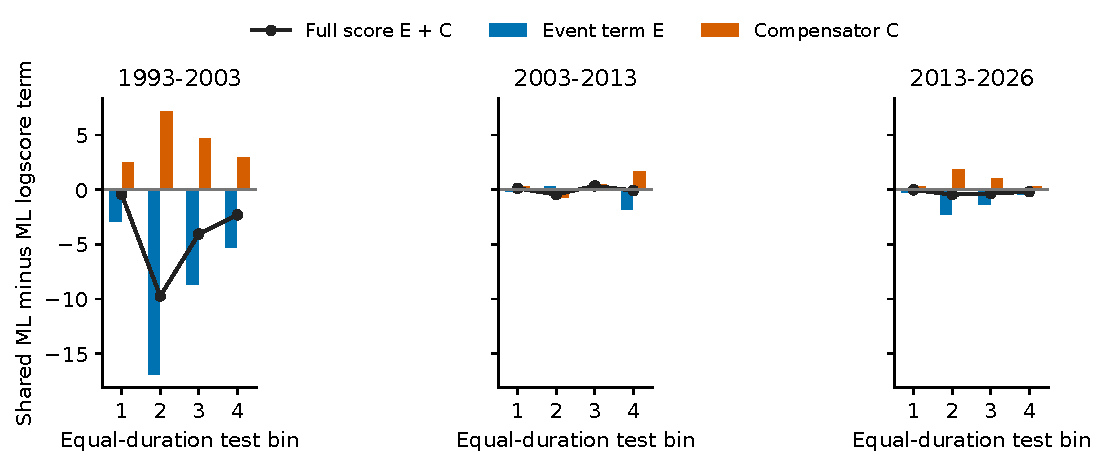
\includegraphics[width=\linewidth]{temporal.pdf}
\caption{Event and compensator contributions in four equal-duration bins in each of the three test periods. Each bin is integrated with complete preceding history. In the first period a favorable compensator contribution partly offsets the negative event term; the full score is their sum.}
\label{fig:temporal}
\end{figure}

A spatial and mark audit found that all five occupied coarse cells had negative event-term contributions for the shared-minus-benchmark contrast. The same direction appeared for native ML and \(M_{\mathrm w}\) magnitude conventions and for all declared magnitude and depth groups. The shared specification contains one regional compensator rather than cell-specific or group-specific exposure. Accordingly, these sums are diagnostics of event-term sign under the fitted family, not local likelihoods, local rates, or fractions of the full score. Unequal cell areas, time-location confounding, sparse cells, and reuse of events across overlapping marginal classifications prevent such a local interpretation. Grouping by the current event's mark is descriptive: that mark affects subsequent intensity and does not enter its own pre-event intensity. Native magnitude-label composition changes most strongly in the last block, whereas the dominant loss is in the first, weakening a simple explanation based only on a modern label transition. Completeness and legacy magnitude-scale concerns remain.

\section{Archive sensitivity and a bounded horizon check}

A replacement audit matched all 913 event identifiers and found 241 numerical magnitude differences, the largest absolute difference being \(0.164143665\). Many differences were only in small decimal places. The full history was rescored using alternate matched magnitudes while primary clocks, locations, depths, the fitted \(\beta\), and the recipe definitions were fixed. The additional event in the 914-event interface selection was excluded, and no parameters were refitted or physically converted between magnitude scales.

Under this replacement, the total shared score changed as follows:
\[
 -17.622859365\ \longrightarrow\ -17.617975447,
 \qquad \text{change }+0.004883918.
\]
No fold changed sign. The Omori total changed from \(12.458121\) to \(12.441651\), shown to six decimal places. Thus the tested archive value discrepancy does not explain the recipe failure. Equally, this bounded audit does not eliminate every observational uncertainty in magnitudes, depths, locations, completeness, or event identity.

A separate horizon-feasibility pilot was restricted and incomplete: 27 of 30 declared horizon-prefix cases completed, one was resource-limited, and two remained pending. Five null paths at a given horizon cannot calibrate a five-percent add-one test: the smallest possible rank is \(1/6\). This is neither a power calculation nor a certificate of sufficient sample size. No incomplete case is treated as a non-rejection, and no resumed or future campaign is claimed. The pilot concerns restricted fitting feasibility. It supplies no calibrated detection decisions or minimum-event requirement.

The observed evidence in this chapter is therefore selective and conditional. The held-out scores are unfavourable to the implemented shared-inhibition recipes, the source-magnitude audit does not reverse that pattern, and the strongest loss is temporally localized. These findings constrain the current diagnostic families. They do not establish the absence of physical shared memory in the Earth system.

The \href{https://github.com/Drefetr/InhibitoryEarthquakeModels/blob/3e76a174cf4f58ce601c6c9640c4d0c11168813f/paper/data/prediction.json}{public predictive summary} and the \hyperref[sec:source-supplements]{availability guide} provide public entry points. Saved summaries do not replace the omitted full authorities or historical history banks.
